\let\negmedspace\undefined
\let\negthickspace\undefined
\documentclass[journal]{IEEEtran}
\usepackage[a5paper, margin=10mm, onecolumn]{geometry}
%\usepackage{lmodern} % Ensure lmodern is loaded for pdflatex
\usepackage{tfrupee} % Include tfrupee package

\setlength{\headheight}{1cm} % Set the height of the header box
\setlength{\headsep}{0mm}     % Set the distance between the header box and the top of the text

\usepackage{gvv-book}
\usepackage{gvv}
\usepackage{cite}
\usepackage{amsmath,amssymb,amsfonts,amsthm}
\usepackage{algorithmic}
\usepackage{graphicx}
\usepackage{textcomp}
\usepackage{xcolor}
\usepackage{txfonts}
\usepackage{listings}
\usepackage{enumitem}
\usepackage{mathtools}
\usepackage{gensymb}
\usepackage{comment}
\usepackage[breaklinks=true]{hyperref}
\usepackage{tkz-euclide} 
\usepackage{listings}
% \usepackage{gvv}                                        
\def\inputGnumericTable{}                                 
\usepackage[latin1]{inputenc}                                
\usepackage{color}                                            
\usepackage{array}                                            
\usepackage{longtable}                                       
\usepackage{calc}                                             
\usepackage{multirow}                                         
\usepackage{hhline}                                           
\usepackage{ifthen}                                           
\usepackage{lscape}
\begin{document}

\bibliographystyle{IEEEtran}
\vspace{3cm}

\title{CHAPTER - 16\\Probability}
\author{EE24BTECH11061 - Rohith Sai}
% \maketitle
% \newpage
% \bigskip
{\let\newpage\relax\maketitle}

\renewcommand{\thefigure}{\theenumi}
\renewcommand{\thetable}{\theenumi}
\setlength{\intextsep}{10pt} % Space between text and floats

\numberwithin{figure}{enumi}
\renewcommand{\thetable}{\theenumi}

\section*{Exercise : 16.3}
\begin{enumerate}
\item [8.1)] Three coins are tossed once, what is the probability of getting three heads?\\
\textbf{Solution:}\\
\textbf{Textual solution: }\\
When three coins are tossed, the sample space is:
\[
S = \{\text{HHH, HHT, HTH, HTT, THH, THT, TTH, TTT}\}
\]
where:
- H represents heads.
- T represents tails.

The total number of outcomes in the sample space is:
\[
|S| = 8
\]

The event \( A \) of getting 3 heads (HHH) contains only one favorable outcome:
\[
A = \{\text{HHH}\}
\]
Thus, the probability of \( A \) is:
\[
P(A) = \frac{\text{Number of favorable outcomes}}{\text{Total number of outcomes}} = \frac{1}{8}
\]

\textbf{Computational solution: }\\

\section*{Introduction}
This document explains the computational process of determining the probability distribution of the number of heads when a coin is tossed three times. The implementation involves two components:
\begin{itemize}
    \item A \textbf{C program} to perform the simulation, calculate the probabilities (PMF), and the cumulative distribution function (CDF).
    \item A \textbf{Python script} to use the results from the C program and generate a plot of the probability.
\end{itemize}

\section*{Definitions}
Let the random variable \( X \) represent the number of heads when three fair coins are tossed. The possible values of \( X \) are:
\[
X \in \{0, 1, 2, 3\}.
\]
\begin{itemize}
    \item \textbf{Probability Mass Function (PMF):} The PMF of \( X \) is defined as:
    \[
    P(X = x) = \frac{\text{Number of occurrences of } x}{\text{Total number of trials}},
    \]
    where \( x \in \{0, 1, 2, 3\} \).
    \item \textbf{Cumulative Distribution Function (CDF):} The CDF of \( X \) is defined as:
    \[
    F(X = x) = \sum_{k=0}^{x} P(X = k),
    \]
    which gives the cumulative probability of obtaining \( k \) or fewer heads.
\end{itemize}

\section*{C Program Implementation}
The C program performs the following steps:
\begin{enumerate}
    \item Simulate \( n \) trials of tossing three coins using the \texttt{rand()} function to generate random outcomes (head or tail).
    \item Count the number of occurrences of 0, 1, 2, and 3 heads across all trials.
    \item Compute the PMF:
    \[
    P(X = x) = \frac{\text{Number of occurrences of } x}{n}, \quad \text{for } x \in \{0, 1, 2, 3\}.
    \]
    \item Compute the CDF using the PMF:
    \[
    F(X = x) = \sum_{k=0}^{x} P(X = k).
    \]
    \item Expose the results (PMF and CDF) as arrays for use in Python.
\end{enumerate}

\section*{Python Script Implementation}
The Python script:
\begin{enumerate}
    \item Loads the shared object file (\texttt{.so}) created by the C program.
    \item Calls the \texttt{calculate\_probabilities} function in the C program, passing the number of trials (\( n \)) and retrieving the PMF and CDF as arrays.
    \item Plots the PMF as a stem plot, showing the probabilities for each outcome (0, 1, 2, and 3 heads).
\end{enumerate}

\section*{Use of CDF in Computation}
The CDF is computed in the C program using the PMF:
\[
F(X = x) = F(X = x-1) + P(X = x), \quad \text{for } x \geq 1,
\]
with the initial condition:
\[
F(X = 0) = P(X = 0).
\]
The Python script does not directly use the CDF but focuses on visualizing the PMF.

\section*{Visualization}
The Python script generates a stem plot of the PMF, illustrating the probabilities for each outcome:
\[
P(X = 0), P(X = 1), P(X = 2), P(X = 3).
\]

\section*{Conclusion}
This computational process combines the efficiency of C for numerical simulation and the versatility of Python for visualization. The CDF plays a key role in ensuring the correctness of cumulative probabilities, which validates the PMF computation.
\begin{figure}[H]
    \centering
    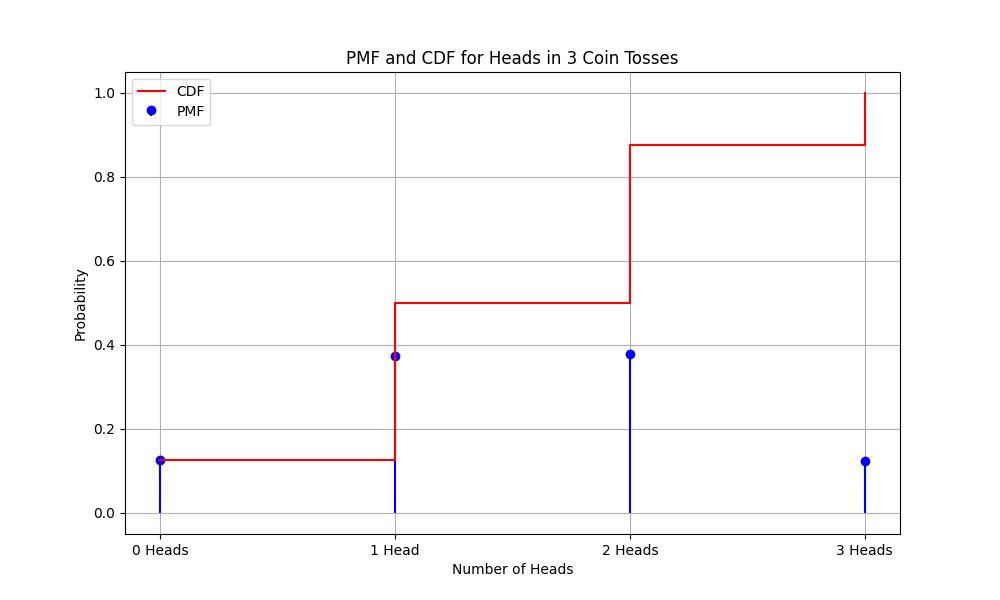
\includegraphics[width=\columnwidth]{figs/fig.png}
\end{figure}
\end{enumerate}
\end{document}